% SPDX-License-Identifier: CC-BY-SA-4.0
% Author: Matthieu Perrin
% Part: 
% Section: 
% Sub-section: 
% Frame: 

\begingroup

\begin{frame}{Grammaire des expressions rationnelles}
  \label{slide:grammaireRegex}
  Soit $\Sigma = \{a, b\}$. Le langage des expressions rationnelles sur $\Sigma$, \\$\textsc{reg}_\Sigma$ est engendré par la grammaire non-ambiguë
  $\langle \tilde\Sigma, \Gamma, \structure{\textsc{Union}}, R \rangle$, où :
  \begin{itemize}
  \item $\tilde\Sigma = \{\example{\underline{a}}, \example{\underline{b}}, \example{\underline{\emptyset}}, \example{\underline{\varepsilon}}, \example{\underline{(}}, \example{\underline{)}}, \example{\underline{|}}, \example{\underline{\cdot}}, \example{\underline{{}^\star}} \}$
  \item $\Gamma = \{\structure{\textsc{Union}}, \structure{\textsc{Concat}}, \structure{\textsc{Etoile}}, \structure{\textsc{Par}}, \structure{\textsc{Terme}}\}$
  \item $R =   \left\{\begin{array}{lllll}
    \structure{\textsc{Union}} &\rightarrow& \structure{\textsc{Union}} \, \example{\underline{|}} \, \structure{\textsc{Concat}} & | &  \structure{\textsc{Concat}} \\
    \structure{\textsc{Concat}} &\rightarrow& \structure{\textsc{Concat}} \, \example{\underline{\cdot}} \, \structure{\textsc{Etoile}} & | & \structure{\textsc{Etoile}} \\
    \structure{\textsc{Etoile}} &\rightarrow& \structure{\textsc{Etoile}}\,^{\example{\underline{\star}}} & | & \structure{\textsc{Par}} \\
    \structure{\textsc{Par}} &\rightarrow&  \example{\underline{(}} \structure{\textsc{Union}} \example{\underline{)}} & | &  \structure{\textsc{Terme}} \\
    \structure{\textsc{Terme}} &\rightarrow& \example{\underline{\varepsilon}} \,|\, \example{\underline{\emptyset}} \,|\, \example{\underline{a}} \,|\, \example{\underline{b}}  \\
  \end{array}\right\}$
  \end{itemize}

  \begin{minipage}[t]{.5\textwidth}
    \begin{block}{Arbre de la syntaxe concrète}
      \scalebox{.5}{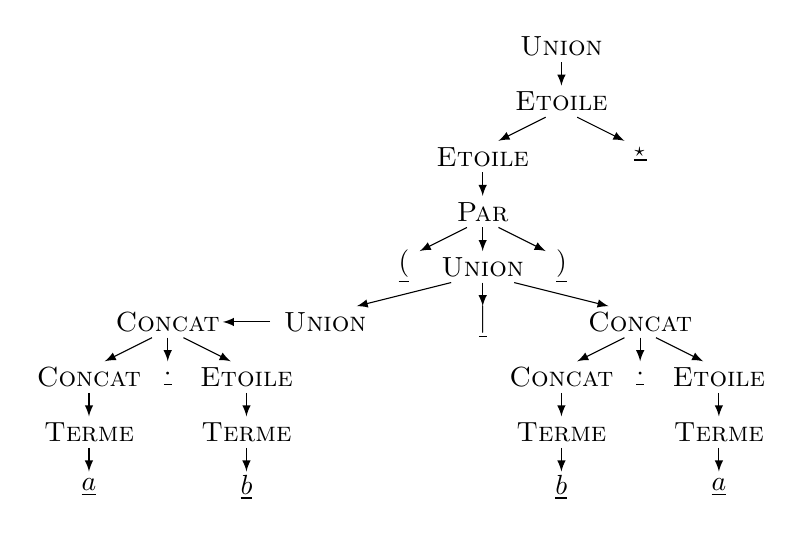
\begin{tikzpicture}
          \draw (6,5.6) node{$\structure{\textsc{Union}}$};
          \draw (6,4.9) node{$\structure{\textsc{Etoile}}$};
          \draw (5,4.2) node{$\structure{\textsc{Etoile}}$};
          \draw (7,4.2) node{${}^{\example{\underline{\star}}}$};
          \draw (5,3.5) node{$\structure{\textsc{Par}}$};
          \draw (4,2.8) node{$\example{\underline{(}}$};
          \draw (5,2.8) node{$\structure{\textsc{Union}}$};
          \draw (6,2.8) node{$\example{\underline{)}}$};
          \draw (1,2.1) node{$\structure{\textsc{Concat}}$};
          \draw (3,2.1) node{$\structure{\textsc{Union}}$};
          \draw (5,2.1) node{$\example{\underline{|}}$};
          \draw (7,2.1) node{$\structure{\textsc{Concat}}$};
          \draw (0,1.4) node{$\structure{\textsc{Concat}}$};
          \draw (1,1.4) node{$\example{\underline{\cdot}}$};
          \draw (2,1.4) node{$\structure{\textsc{Etoile}}$};
          \draw (6,1.4) node{$\structure{\textsc{Concat}}$};
          \draw (7,1.4) node{$\example{\underline{\cdot}}$};
          \draw (8,1.4) node{$\structure{\textsc{Etoile}}$};
          \draw (0,0.7) node{$\structure{\textsc{Terme}}$};
          \draw (2,0.7) node{$\structure{\textsc{Terme}}$};
          \draw (6,0.7) node{$\structure{\textsc{Terme}}$};
          \draw (8,0.7) node{$\structure{\textsc{Terme}}$};
          \draw (0,0.0) node{$\example{\underline{a}}$};
          \draw (2,0.0) node{$\example{\underline{b}}$};
          \draw (6,0.0) node{$\example{\underline{b}}$};
          \draw (8,0.0) node{$\example{\underline{a}}$};
          
          \draw[-latex] (6.0,5.4) -- (6.0,5.1);
          \draw[-latex] (5.8,4.7) -- (5.2,4.4);
          \draw[-latex] (6.2,4.7) -- (6.8,4.4);
          \draw[-latex] (5.0,4.0) -- (5.0,3.7);
          \draw[-latex] (4.8,3.3) -- (4.2,3.0);
          \draw[-latex] (5.0,3.3) -- (5.0,3.0);
          \draw[-latex] (5.2,3.3) -- (5.8,3.0);
          \draw[-latex] (2.3,2.1) -- (1.7,2.1);
          \draw[-latex] (4.6,2.6) -- (3.4,2.3);
          \draw[-latex] (5.0,2.6) -- (5.0,2.3);
          \draw[-latex] (5.4,2.6) -- (6.6,2.3);
          \draw[-latex] (0.8,1.9) -- (0.2,1.6);
          \draw[-latex] (1.0,1.9) -- (1.0,1.6);
          \draw[-latex] (1.2,1.9) -- (1.8,1.6);
          \draw[-latex] (6.8,1.9) -- (6.2,1.6);
          \draw[-latex] (7.0,1.9) -- (7.0,1.6);
          \draw[-latex] (7.2,1.9) -- (7.8,1.6);
          \draw[-latex] (0.0,1.2) -- (0.0,0.9);
          \draw[-latex] (2.0,1.2) -- (2.0,0.9);
          \draw[-latex] (6.0,1.2) -- (6.0,0.9);
          \draw[-latex] (8.0,1.2) -- (8.0,0.9);
          \draw[-latex] (0.0,0.5) -- (0.0,0.2);
          \draw[-latex] (2.0,0.5) -- (2.0,0.2);
          \draw[-latex] (6.0,0.5) -- (6.0,0.2);
          \draw[-latex] (8.0,0.5) -- (8.0,0.2);
      \end{tikzpicture}}
    \end{block}
  \end{minipage}%
  \begin{minipage}[t]{.5\textwidth}
    \begin{block}{Arbre de la syntaxe abstraite}
      \scalebox{.75}{\begin{tikzpicture}
          \draw (3.0,3.0) node{${}^{\example{\underline{\star}}}$};
          \draw (3.0,2.0) node{$\example{\underline{|}}$};
          \draw (1.0,1.0) node{$\example{\underline{\cdot}}$};
          \draw (5.0,1.0) node{$\example{\underline{\cdot}}$};
          \draw (0.0,0.0) node{$\example{\underline{a}}$};
          \draw (2.0,0.0) node{$\example{\underline{b}}$};
          \draw (4.0,0.0) node{$\example{\underline{b}}$};
          \draw (6.0,0.0) node{$\example{\underline{a}}$};

          \draw[-latex] (3.0,2.8) -- (3.0,2.3); 
          \draw[-latex] (2.6,1.8) -- (1.4,1.2); 
          \draw[-latex] (3.4,1.8) -- (4.6,1.2); 
          \draw[-latex] (0.8,0.8) -- (0.2,0.2); 
          \draw[-latex] (1.2,0.8) -- (1.8,0.2); 
          \draw[-latex] (4.8,0.8) -- (4.2,0.2); 
          \draw[-latex] (5.2,0.8) -- (5.8,0.2); 
      \end{tikzpicture}}
    \end{block}
  \end{minipage}
\end{frame}
\endgroup
